\documentclass[10pt]{article}

\usepackage{spheric}
%%%TITLE
\title{Application of particle-based computational acoustics to sound propagation and scattering}
\date{}

%%AFFILIATIONS
\author[$\relax$]{Yong Ou ZHANG$^\dagger$}

\affil[$\relax$]{School of Transportation, Wuhan University of Technology, China}

\affil[$\relax$]{\email{\dagger}{zhangyo@whut.edu.cn}}


%%DOCUMENT
\begin{document}

\maketitle

%\SelectedTopics{}

%%PLEASE PUT YOUR ABSTRACT HERE
\begin{abstract}
The Lagrangian meshfree method with interacting particles is a powerful and natural approach for simulating physical systems with complicated domain topologies, moving boundaries, and multiphase media. Particle-based computational acoustics (PCA), as a noval branch of computational acoustics, aims to simulate acoustic phenomenon by Lagrangian meshfree particle methods. The ability of different particle methods to simulate flow-acoustic and flow-structure-acoustic interaction problems is evaluated. To separate the acoustic perturbation from the particle motion, Lagrangian acoustic perturbation equations (LAPE) including two sets of governing equations are used. Smoothed particle hydrodynamics (SPH), corrective smoothed particle method (CSPM), and finite difference particle method (FDPM) are selected for a comparison. Several checks on the accuracy and convergence of the Lagrangian meshfree PCA method are discussed. Numerical results are obtained for various sound propagation and scattering problems, and different acoustic boundary conditions including perfectly matched layers are examined.

\begin{figure}[!htb]
\centering
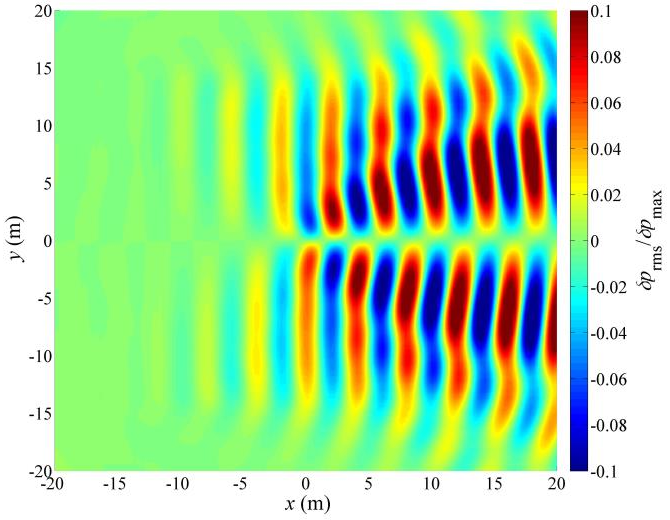
\includegraphics[width=0.65\textwidth]{54-1.png}
\caption{Non-dimensional sound pressure of vortex scattering at $\mathrm{Ma} = 0.2$}\label{fig:}
\end{figure}

\end{abstract}


%%THE END OF ABSTRACT

%\addbib

\end{document}
